% Compact PGFPlots panel for sampled surface7 depolarizing GEXIT derivative.
% Requires \usepackage{pgfplots} and \pgfplotsset{compat=1.18}.
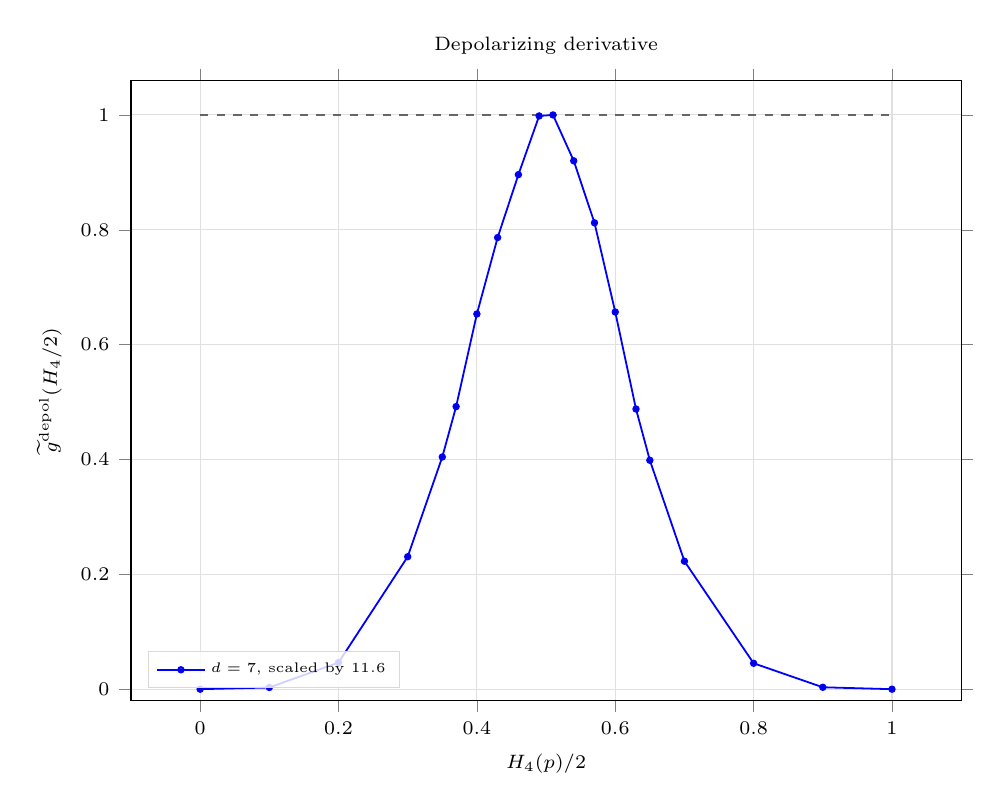
\begin{tikzpicture}
\begin{axis}[
  name=scaledDepolarizingGEXITSurface7Axis,
  width=\linewidth,
  height=0.78\linewidth,
  title={Depolarizing derivative},
  title style={font=\scriptsize},
  xlabel={$H_4(p)/2$},
  ylabel={$\widetilde g^{\rm depol}(H_4/2)$},
  ymin=-0.02, ymax=1.06,
  grid=both,
  major grid style={black!12},
  minor grid style={black!6},
  tick align=outside,
  tick label style={font=\scriptsize},
  label style={font=\scriptsize},
  legend cell align={left},
  legend style={draw=black!15, fill=white, fill opacity=0.82, text opacity=1, at={(0.02,0.02)}, anchor=south west, font=\tiny},
]
\addplot[black!60, dashed, line width=0.55pt, forget plot] coordinates {(0,1) (1,1)};
\addplot+[color=blue, mark=*, mark size=1.0pt, line width=0.65pt]
coordinates {(0,0) (0.1,0.00295645955089) (0.2,0.0463368250444) (0.3,0.230674423002) (0.35,0.404356116017) (0.37,0.492124430801) (0.4,0.653376106363) (0.43,0.786462010477) (0.46,0.896005711653) (0.49,0.998262837311) (0.51,1) (0.54,0.920114970537) (0.57,0.812139542886) (0.6,0.656859913063) (0.63,0.487919909896) (0.65,0.398650257397) (0.7,0.22283287194) (0.8,0.0451166562625) (0.9,0.00332813163872) (1,0)};
\addlegendentry{$d=7$, scaled by $11.6$}
\end{axis}
\end{tikzpicture}
